\section{Auswertung}
\label{sec:Auswertung}

\subsection{Wheatstone Brücke}
\begin{table}[H]
    \centering
    \caption{Werte der Widerstände zur Wheatstone Brücke.}
    \label{tab:t1}
    \begin{tabular}{|l|c|c|c|}
        \hline
        & \textbf{$R_2$ / $\Omega$} & \textbf{$R_3$ / $\Omega$} & \textbf{$R_4$ / $\Omega$} \\
        \hline
        %\multicolumn{4}{|l|}{\textbf{Daten von "Wert 10"}} \\
        \hline
               & 1000 & 330 & 670 \\
        Wert11 & 664  & 426 & 574 \\
               & 332  & 597 & 403 \\
        \hline
        %\multicolumn{4}{|l|}{\textbf{Daten von "Wert 11"}} \\
        \hline
               & 1000 & 474 & 526 \\
        Wert14 & 664  & 574 & 426 \\
               & 332  & 732 & 268 \\
        \hline
        \hline
               & 1000 & 281 & 719 \\
        Wert12 & 664  & 370 & 630 \\
               & 332  & 541 & 459 \\
        \hline
    \end{tabular}
\end{table}


\subsection{Kapazitätsmessbrücke}
\begin{table}[H]
  \centering
  \caption{Werte der Widerstände zur Kapazitätsmessbrücke.}
  \label{tab:t2}
  \begin{tabular}{|l|c|c|c|c|}
      \hline
      & \textbf{$C_2$ / \unit{\nF}} & \textbf{$R_2$ / $\Omega$} & \textbf{$R_3$ / $\Omega$} & \textbf{$R_4$ / $\Omega$} \\
      \hline
      %\multicolumn{4}{|l|}{\textbf{Daten von "Wert 10"}} \\
      \hline
            & 992 & 164 & 772 & 228 \\
      Wert8 & 450 & 369 & 603 & 397 \\
            & 597 & 728 & 670 & 330 \\
      \hline
      %\multicolumn{4}{|l|}{\textbf{Daten von "Wert 11"}} \\
      \hline
             & 992 & 285 & 620 & 380 \\
      Wert15 & 450 & 654 & 413 & 587 \\
             & 597 & 542 & 471 & 529 \\
      \hline
      \hline
            & 992 & 204 & 693 & 307 \\
      Wert9 & 450 & 443 & 510 & 490 \\
            & 597 & 334 & 580 & 420 \\
      \hline
  \end{tabular}
\end{table}

\subsection{Induktivitätsmessbrücke}
\begin{table}[H]
  \centering
  \caption{Werte der Widerstände zur Induktivitätsmessbrücke.}
  \label{tab:t3}
  \begin{tabular}{|l|c|c|c|c|}
      \hline
      & \textbf{$L_2$ / \unit{\mH}} & \textbf{$R_2$ / $\Omega$} & \textbf{$R_3$ / $\Omega$} & \textbf{$R_4$ / $\Omega$} \\
      \hline
      %\multicolumn{4}{|l|}{\textbf{Daten von "Wert 10"}} \\
      \hline
             & 14.6 & 58  & 647 & 353 \\
      Wert19 & 27.5 & 108 & 496 & 504 \\
             & 20.1 & 75  & 572 & 428 \\
      \hline
      %\multicolumn{4}{|l|}{\textbf{Daten von "Wert 11"}} \\
      \hline
             & 14.6 & 51 & 901 & 99  \\
      Wert16 & 27.5 & 86 & 831 & 169 \\
             & 20.1 & 59 & 870 & 130 \\
      \hline
      \hline
             & 14.6 & 103 & 773 & 227 \\
      Wert18 & 27.5 & 194 & 645 & 355 \\
             & 20.1 & 138 & 713 & 287 \\
      \hline
  \end{tabular}
\end{table}

\subsection{Wien-Robinson Messbrücke}
% \begin{longtblr}[caption = {Wien-Robinson Messbrücke}]{
%     colspec = {S S },
%     row{1} = {guard, mode=math},
%     vline{2} = {2}{-}{text=\clap{$\pm$}},
%     vline{4} = {2}{-}{text=\clap{$\pm$}},
%     %vline{4} = {2}{-}{text=\clap{$\pm$}},
%     }
%     \toprule
%     \SetCell[c=2]{c} \nu /\unit{\Hz}& &\SetCell[c=2]{c} U/\unit{\mV} \\
%     \midrule
%     50   & 300 \\
%     70   & 260 \\
%     90   & 230 \\
%     110  & 190 \\
%     130  & 150 \\
%     150  & 115 \\
%     170  & 80  \\
%     190  & 55  \\
%     210  & 35  \\
%     230  & 10  \\
%     250  & 10  \\
%     270  & 27  \\
%     290  & 44  \\
%     310  & 60  \\
%     330  & 70  \\
%     350  & 85  \\
%     370  & 100 \\
%     390  & 110 \\
%     410  & 120 \\
%     430  & 130 \\
%     450  & 140 \\
%     470  & 150 \\
%     490  & 160 \\
%     510  & 170 \\
%     530  & 175 \\
%     550  & 180 \\
%     570  & 185 \\
%     590  & 195 \\
%     610  & 200 \\
%     630  & 210 \\
%     650  & 215 \\
%     670  & 225 \\
%     690  & 230 \\
%     710  & 230 \\
%     730  & 225 \\
%     750  & 240 \\
%     770  & 245 \\
%     790  & 250 \\
%     810  & 245 \\
%     830  & 250 \\
%     850  & 250 \\
%     870  & 255 \\
%     890  & 250 \\
%     910  & 255 \\
%     930  & 260 \\
%     950  & 265 \\
%     970  & 265 \\
%     990  & 270 \\
%     1100 & 275 \\
%     \bottomrule
%   \end{tblr}
% \end{table}

\subsection{Wien-Robinson Messbrücke}
Mit hilfe der Wien-Robinson Messbrücke kann der Klirrfaktor der Speisespannung ermittelt 
werden. Dazu tragen wir in einem halblogarythmischen Diagramm Die Brückenspannung, bzw das 
verhältnis der Brückenspannung zur Speisespannung $(\frac{U_{Br}}{U_s})$, in abhängigkeit von 
der Frequenz $\omega$ auf.
\begin{figure}
       \caption{Verhältnis Brückenspannung zu Speisespannung abhängig von der Frequenz und errechnete Funktion}
       \label{fig:ub}
       \centering
       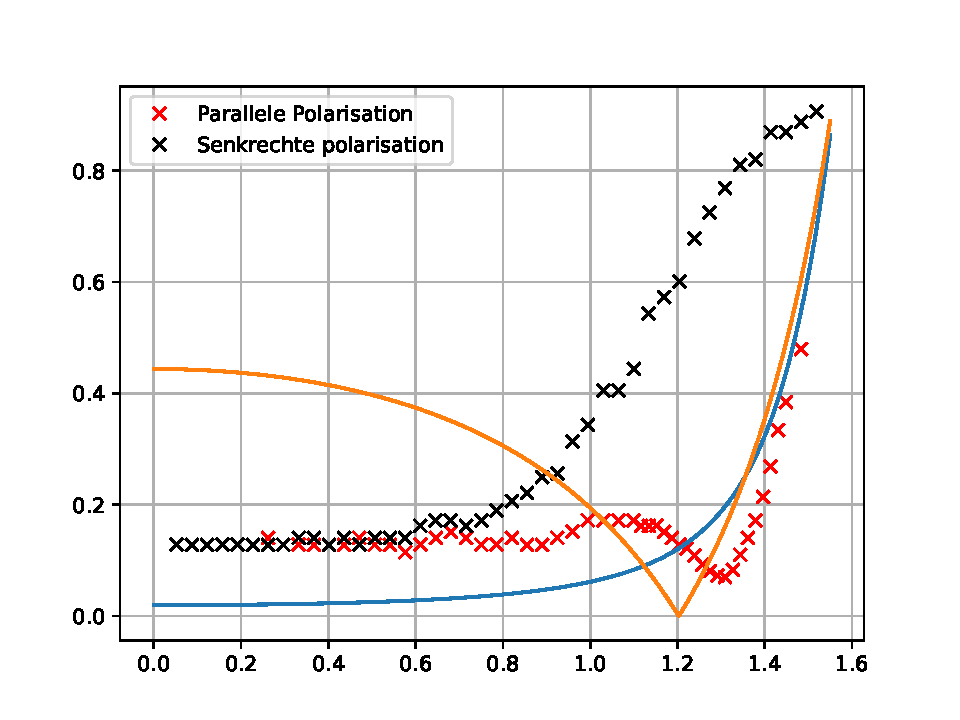
\includegraphics{"build/plot.pdf"}
\end{figure}
Die Messwerte für $\frac{U_{Br}}{U_s}\left(\omega\right)$ in \autoref{fig:ub}
